\documentclass[10pt]{ctexart}
\usepackage[colorlinks=true]{hyperref}
\usepackage{amsmath}
\usepackage{graphicx}
\usepackage{esint}
\usepackage{float}
\usepackage{ulem}
\usepackage{geometry}
\usepackage{booktabs}
\usepackage{multirow}
\usepackage{esint}
\setCJKmainfont{HarmonyOS Sans SC}
%\geometry{a5paper,left=2cm,right=2cm,top=1cm,bottom=1cm}
\geometry{a5paper,scale=0.9}
\pagestyle{empty}
\author{树影、九鸟}
\title{大雾二寄结论速寄2}
\date{}

\begin{document}
\maketitle
\newpage
\tableofcontents
\newpage
\section*{前言}

上一次的笔记就说明了,这玩意只有复习作用,不代表考试会考()。依然不会对内容正确性负责。

\section{热力学}
\label{sec:热力学}

\subsection{理想气体、(热力学定律:theorems list)[0]}
\label{subsec:理想气体、(热力学定律:theorems list)[0]}

理想气体状态方程常见的形式如下:
\begin{align*}
    p V &= N k T \\
    p V &= \mu R T \\
    p &= n k T \\
    p M &= \rho R T
\end{align*}

符号解释(符号都请与高中的区别开来,不要混淆,虽然对我而言是一件痛苦的事):

\begin{table}[H]
    \centering
    \begin{tabular}{l|c}
        符号 & 含义 \\
        \hline
        $p$ & 压强 \\
        $V$ & 体积 \\
        $N$ & 分子数 \\
        $k$ & 玻尔兹曼常数 \\
        $T$ & 温度 \\
        $\mu$ & 气体分子的物质的量 \\
        $R$ & 摩尔气体常数 \\
        $n$ & 气体分子数密度 \\
        $M$ & 气体的分子量 \\
        $\rho$ & 气体的密度
    \end{tabular}
\end{table}

\begin{align*}
    k &= 1.38 \times 10^{-23} \, \text{J/K} \\
    R &= 8.31 \, \text{J/(mol K)} \\
    R = k N_A &= 8.31 \, \text{J/(mol K)} \\
\end{align*}

热力学定律[0]: 如果物体A与物体B处于热平衡状态,物体A与物体C也处于热平衡状态,则物体B与物体C也处于热平衡状态。

\subsection{物质的微观模型,统计规律}
\label{subsec:物质的微观模型,统计规律}

\begin{figure}[H]
    \centering
    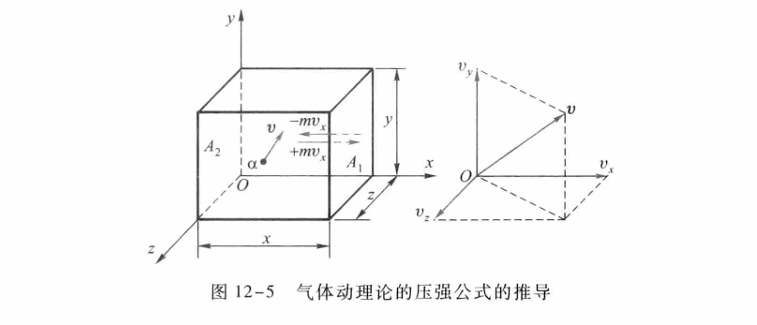
\includegraphics[width=0.8\textwidth]{img/12/1.png}
\end{figure}

要点:
\begin{itemize}
    \item [0.] 对于$A_1$面,两次碰撞的时间间隔为:$2 \frac{x}{v_x}$,$v_x$为分子在$x$方向的速度。
    \item [1.] 对于$A_1$面,单位时间内碰撞,一个分子对于$A_1$面的冲量为:$2 m v_x \cdot \frac{v_x}{2 x}$,$m$为分子质量。
    \item [2.] 作用于$A_1$面上的力为:$F = \sum_{i=1}^{N} 2 m v_{x_i} \cdot \frac{v_{x_i}}{2 x} = \frac{\sum_{i=1}^{N} m v_{x_i}^2 }{x}$,$N$为分子数。
    \item [3.] 作用于$A_1$面上的压强为:$p = \frac{F}{S} = \frac{\sum_{i=1}^{N} m v_{x_i}^2}{xyz} = \frac{Nm\bar{v_x^2}}{V} = n m \bar{v_x^2}$.
\end{itemize}

由最后的一步,根据$x y z$的对称性,可以得到$3 p = n m \bar{v^2}$,其中$\bar{v^2}$为分子平均速度的平方。

即:
$$
    p = \frac{1}{3} n m \bar{v^2}
$$

若令$\bar{\varepsilon_k} = \frac{1}{2} m \bar{v^2}$,则有:
$$
    p = \frac{2}{3} n \bar{\varepsilon_k}
$$

$\varepsilon_k$为分子的平均平动动能。

将其与理想气体状态方程联立,得到:
$$
    \bar{\varepsilon_k} = \frac{3}{2} k T
$$

又有$ n m = \rho $ ,则有:
$$
    p = \frac{2}{3} \rho \bar{v^2}
$$

由:$\bar{\varepsilon_k} = \frac{3}{2} k T$可知,对于分别处于相同温度的两种气体,其分子的平均平动动能相同。

\subsection{能量均分定理}
\label{subsec:能量均分定理}

定义将分子能量中速度和坐标的二次项数目叫做分子能量的自由度数目,简称为自由度,用符号 $i$ 表示。

能量均分定理的内容为:在平衡状态下,每个自由度平均能量均相等,且为:为 $\frac{1}{2} k T$。

\begin{figure}[H]
    \centering
    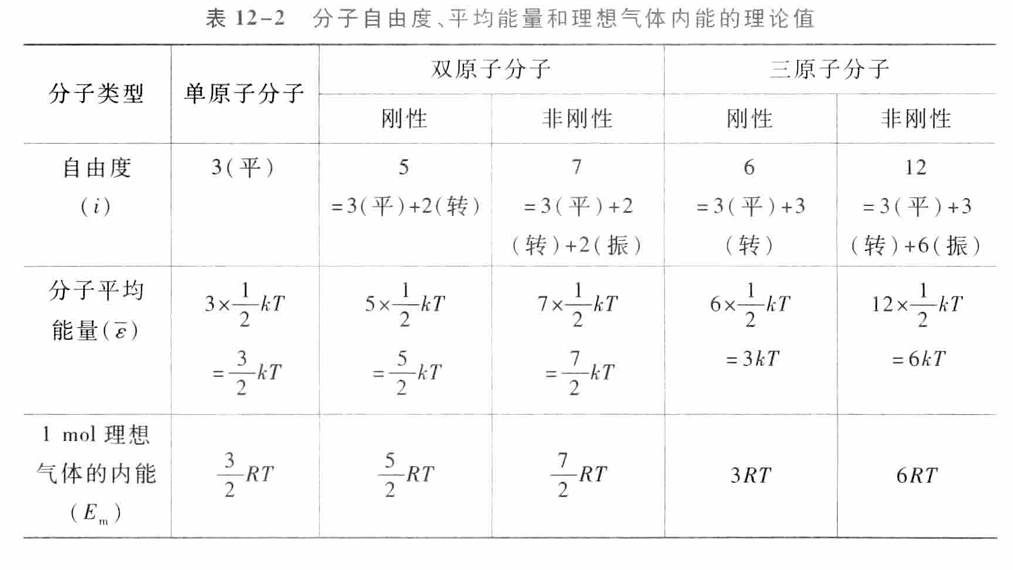
\includegraphics[width=0.8\textwidth]{img/12/2.png}
    \caption{常见气体分子的自由度以及平均能量}
\end{figure}

\subsection{麦克斯韦速率分布定律}
\label{subsec:麦克斯韦速率分布定律}

对于分布在速度区间 $v$ 到 $v + d v$ 的分子的概率:

$$
    \frac{d N}{N} = 4 \pi \left( \frac{m}{2 \pi k T} \right)^{3/2} v^2 e^{-\frac{m v^2}{2 k T}} d v
$$

推导:

不难得到:理想气体分子的速度分布有:
\begin{align*}
    v_x &\sim N(0, \sigma^2) \\
    v_y &\sim N(0, \sigma^2) \\
    v_z &\sim N(0, \sigma^2)
\end{align*}

得速度的联合分布为:
$$
    f(v_x,v_y,v_z) = \frac{1}{(2 \pi \sigma^2)^{3/2}} e^{-\frac{v_x^2 + v_y^2 + v_z^2}{2 \sigma^2}}
$$

所以速率分布为:
$$
    f(v) = \oiint_{\Sigma:v_x^2 + v_y^2 + v_z^2 = v^2} v(v_x,v_y,v_z) d v_x d v_y d v_z
$$
$$
    f(v) = 4\pi v^2 \frac{1}{(2 \pi \sigma^2)^{3/2}} e^{-\frac{v^2}{2 \sigma^2}}
$$

而$\sigma$ 可以通过平均平动动能来计算:
$$
    E(v_x^2) =\sigma^2= \frac{2\bar{\varepsilon_x}}{m} = \frac{kT}{m}
$$

\subsection{三种统计速率}
\label{subsec:三种统计速率}

方均根速率、平均速率、最概然速率:
\begin{align*}
    v_{\text{rms}} &= \sqrt{\bar{v^2}} = \sqrt{\frac{3kT}{m}} \\
    v_{\text{avg}} &= E(v) = \sqrt{\frac{8kT}{\pi m}} \\
    v_{\text{mp}} &= \sqrt{\frac{2kT}{m}}
\end{align*}

% v_{\text{rms}} 是采用 \sqrt{\bar{v^2}} 计算,而\bar{v^2} 是一个无偏统计量,但是 v_{rms} 不是无偏估计.
% 由根号函数的性质,其右偏,故 v_{\text{rms}} > v_{\text{avg}}。
% 而f(v) 是一个左偏分布,故 v_{\text{mp}} < v_{\text{avg}}。

大小关系:由于 $v_{\text{rms}} > v_{\text{avg}} > v_{\text{mp}}$,所以在速率分布图上,$v_{\text{rms}}$ 在 $v_{\text{avg}}$ 和 $v_{\text{mp}}$ 之间。

\subsection{玻尔兹曼能量分布定律}
\label{subsec:玻尔兹曼能量分布定律}

麦克斯韦速率分布可以改写为:
$$
    d N = N \left( \frac{m}{2 \pi k T} \right)^{3/2} e^{-\frac{\varepsilon_k}{k T}} d v
$$

在还存在势场的情况下,玻尔兹曼认为应该用$\varepsilon_k + \varepsilon_p$来代替$\varepsilon_k$,从这个角度,他得到了分子数关于速度与位置的分布:
$$
    d N_{v_x,v_y,v_z,x,y,z} = n_0 \left( \frac{m}{2 \pi k T} \right)^{3/2} e^{-\frac{\varepsilon_k + \varepsilon_p}{k T}} d v_x d v_y d v_z d x d y d z
$$

$n_0$ 表示势能为零时的分子数密度。

对上式对速度积分,得到:
$$
    d N_{x,y,z} = n_0 e^{-\frac{\varepsilon_p}{k T}} d x d y d z
$$

即:
$$
    n = n_0 e^{-\frac{\varepsilon_p}{k T}}
$$

在地球表面,$\varepsilon_p = mgh$,所以:
$$
    n = n_0 e^{-\frac{mgh}{k T}}
$$

假如认为地球大气是等温的,并且忽略地球引力的变化,那么可以得到重力场中的等温气压分布:
$$
    p = p_0 e^{-\frac{mgh}{k T}}
$$

由此便可以进行高度估计:
$$
    h = \frac{k T}{m g} \ln \frac{p_0}{p} = \frac{R T}{M g} \ln \frac{p_0}{p}
$$

\subsection{分子之间的碰撞频率与平均自由程}
\label{subsec:分子之间的碰撞频率与平均自由程}

分子之间的平均碰撞频率为:
$$
    \bar{Z} = \sqrt{2} \pi d^2 \bar{v} n
$$

其中 $d$ 为分子直径,$n$ 为分子数密度,$\bar{v}$ 为分子平均速率。

而平均自由程可以表示为:
$$
    \bar{\lambda} = \frac{\bar{v}}{\bar{Z}} = \frac{1}{\sqrt{2}\pi d^2 n}
$$

由于$p = nkT$,所以可以得到:
$$
    \bar{\lambda} = \frac{kT}{\sqrt{2}\pi d^2 p}
$$
\end{document}